\subsection{S+P Results}
\label{resultssec:sp}

Fig.~\ref{fig:sp_parametric} shows, for each squared dataset, the average PSNR
(in dB) as a function of the average compression ratio (CR) obtained by sweeping
the S+P quantization scale. As expected, all four curves exhibit a monotone
tradeoff: increasing CR is accompanied by decreasing PSNR. The datasets,
however, occupy different regions of the CR axis. Kodak, AerialImages, and
TextureImages all span roughly CR~$\approx 2$--$8$, whereas IconsSample is
confined to about CR~$\approx 1.7$--$6$, reflecting that these very small,
simple images cannot be pushed to the same nominal compression ratios.
\begin{figure}
    \centering
    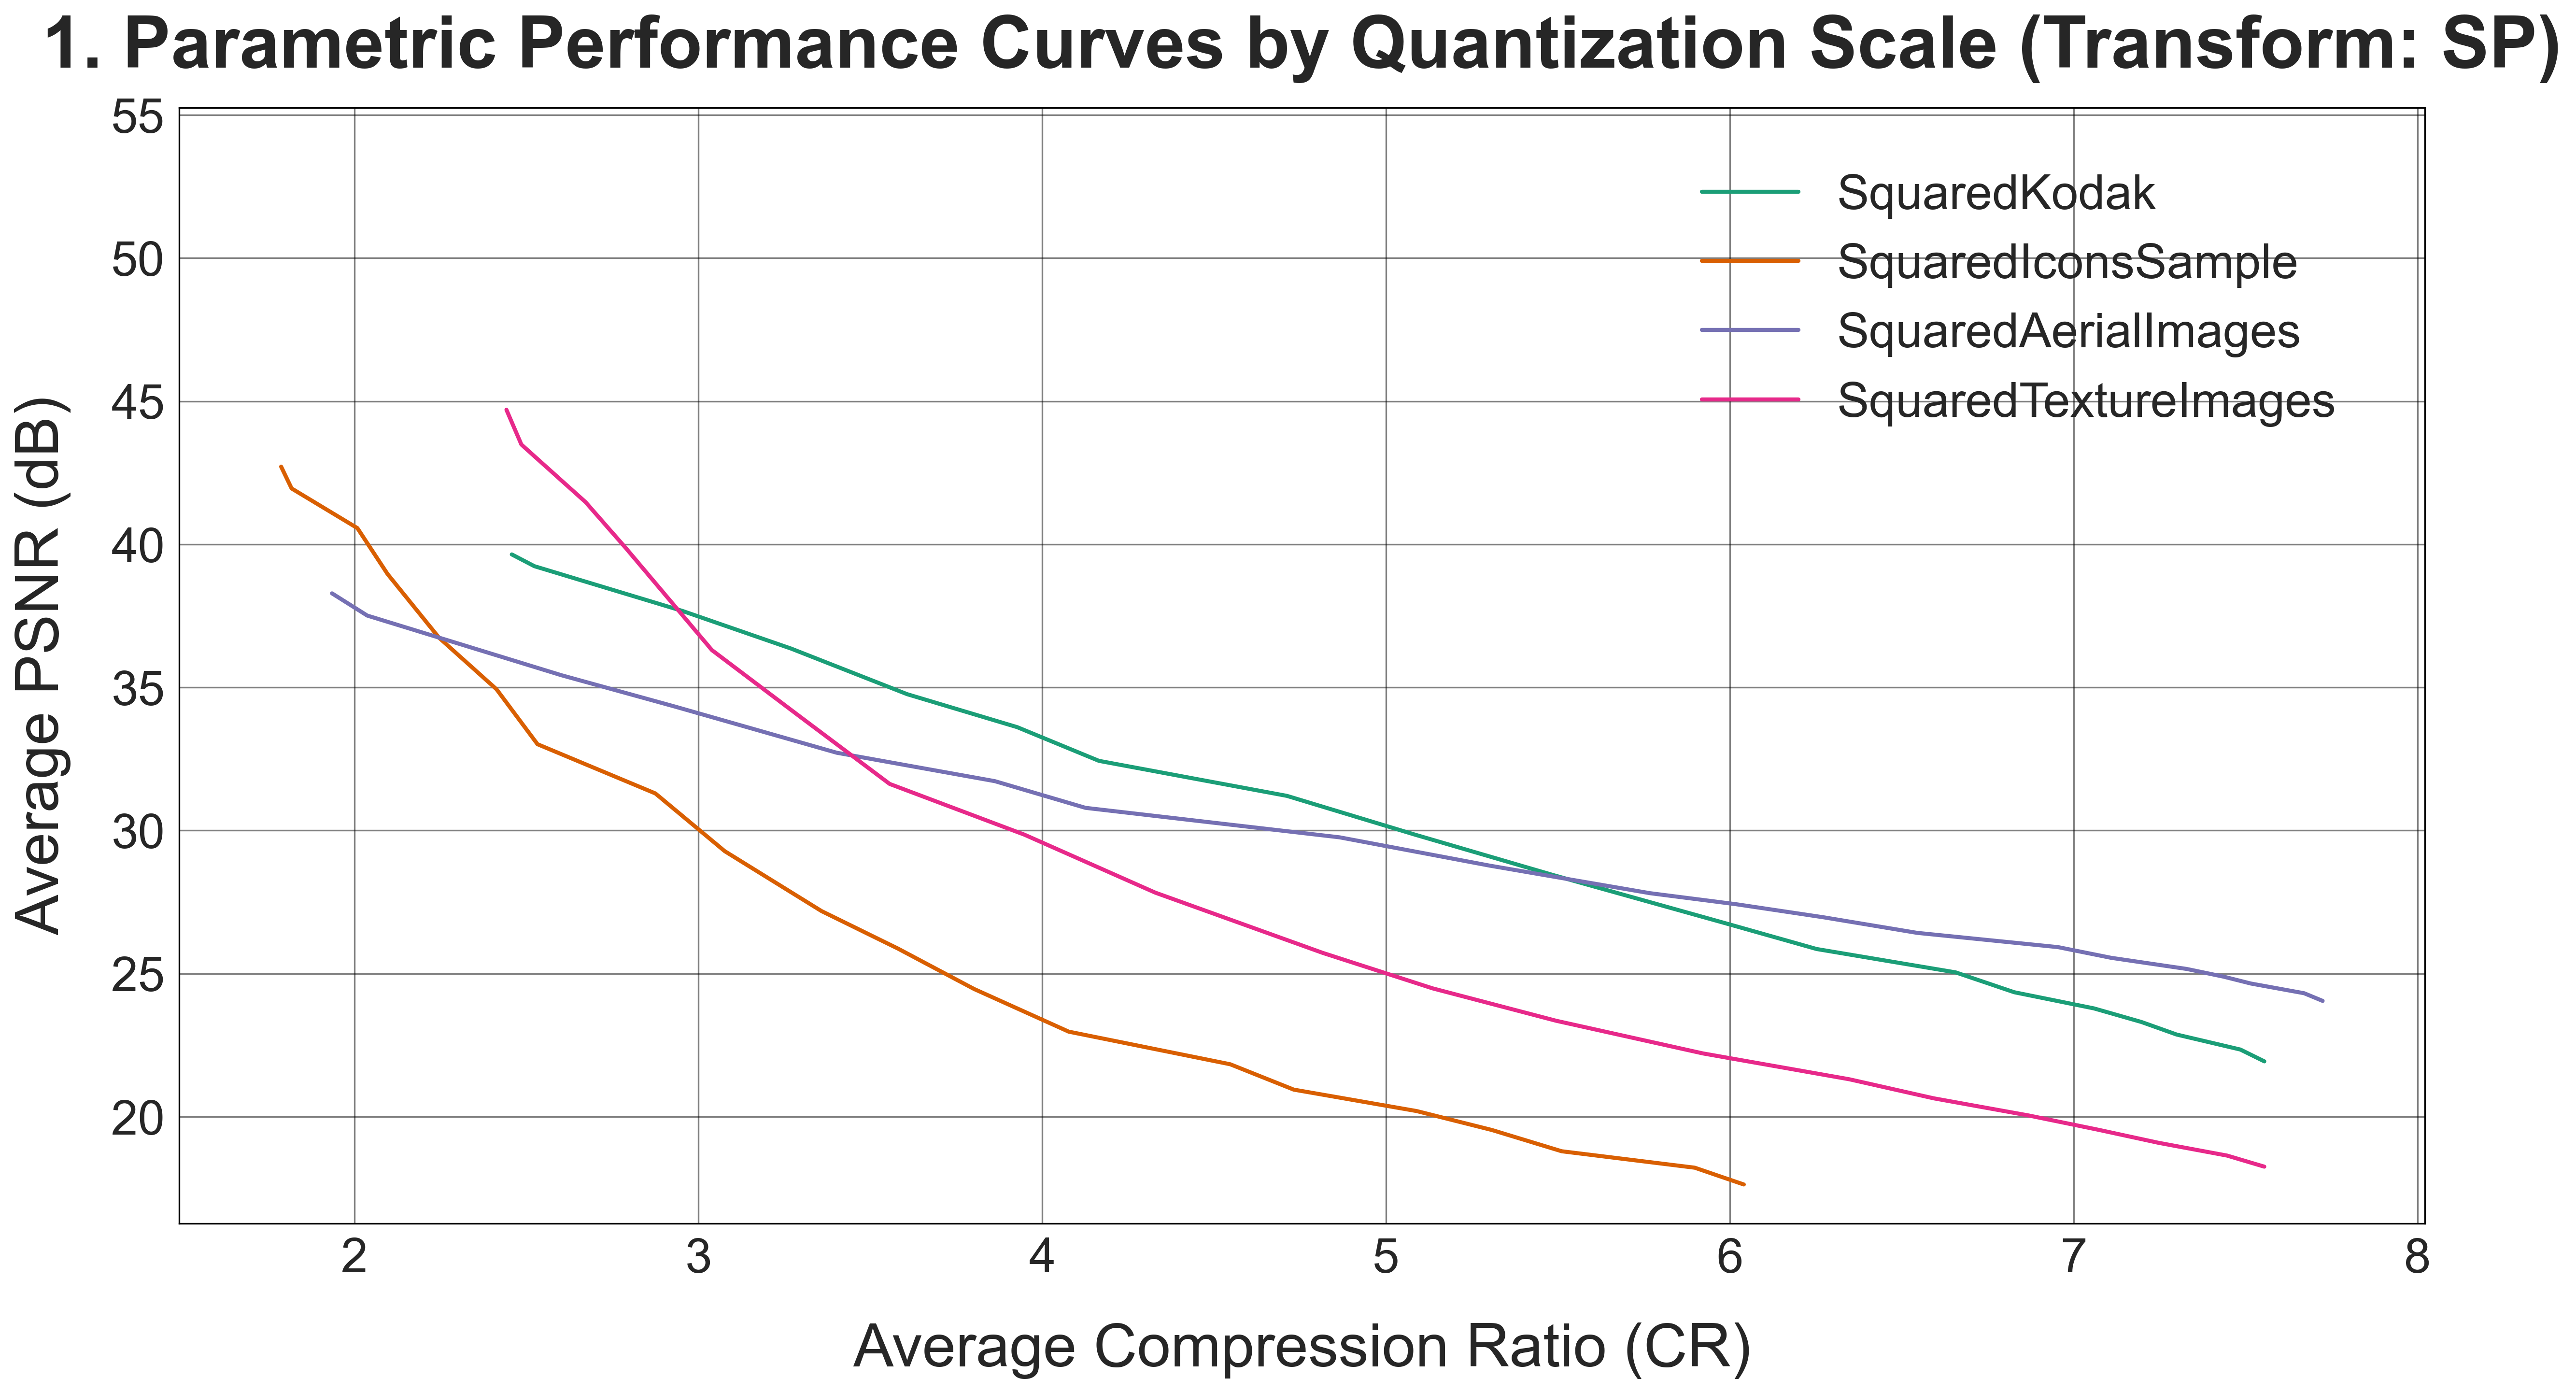
\includegraphics[width=1\linewidth]{results/plots/plot_1_parametric_curve_SP.png}
    \caption{S+P parametric performance: average PSNR vs.\ average compression ratio.}
    \label{fig:sp_parametric}
\end{figure}
At the low-CR end (around CR~$\approx 2$), TextureImages achieves the highest
average PSNR (around 45\,dB), with IconsSample close behind, and Kodak and
AerialImages clustered around 38--39\,dB. As CR increases, all curves slope
downward, but with noticeably different steepness. The Kodak and AerialImages
curves remain relatively close together, maintaining PSNR in the low
30\,dB range at CR~$\approx 4$ and still above 25\,dB at CR~$\approx 7$.
TextureImages falls somewhat faster but stays competitive through most of the
range. IconsSample begins near the top-left of the plot with high PSNR at
low CR, but its curve is the steepest: by CR~$\approx 5$ it has dropped to
around 20\,dB, and it does not extend into the very high-CR regime where the
other datasets continue.

Overall, these curves show that S+P exhibits the same dataset ordering
we observed in the Collective Results, with natural-image datasets clustering
together and IconsSample behaving as a low-CR, high-PSNR regime.
% providing a
% clear baseline for our direct comparison between S+P and Haar in the next
% section.

\begin{figure}
    \centering
    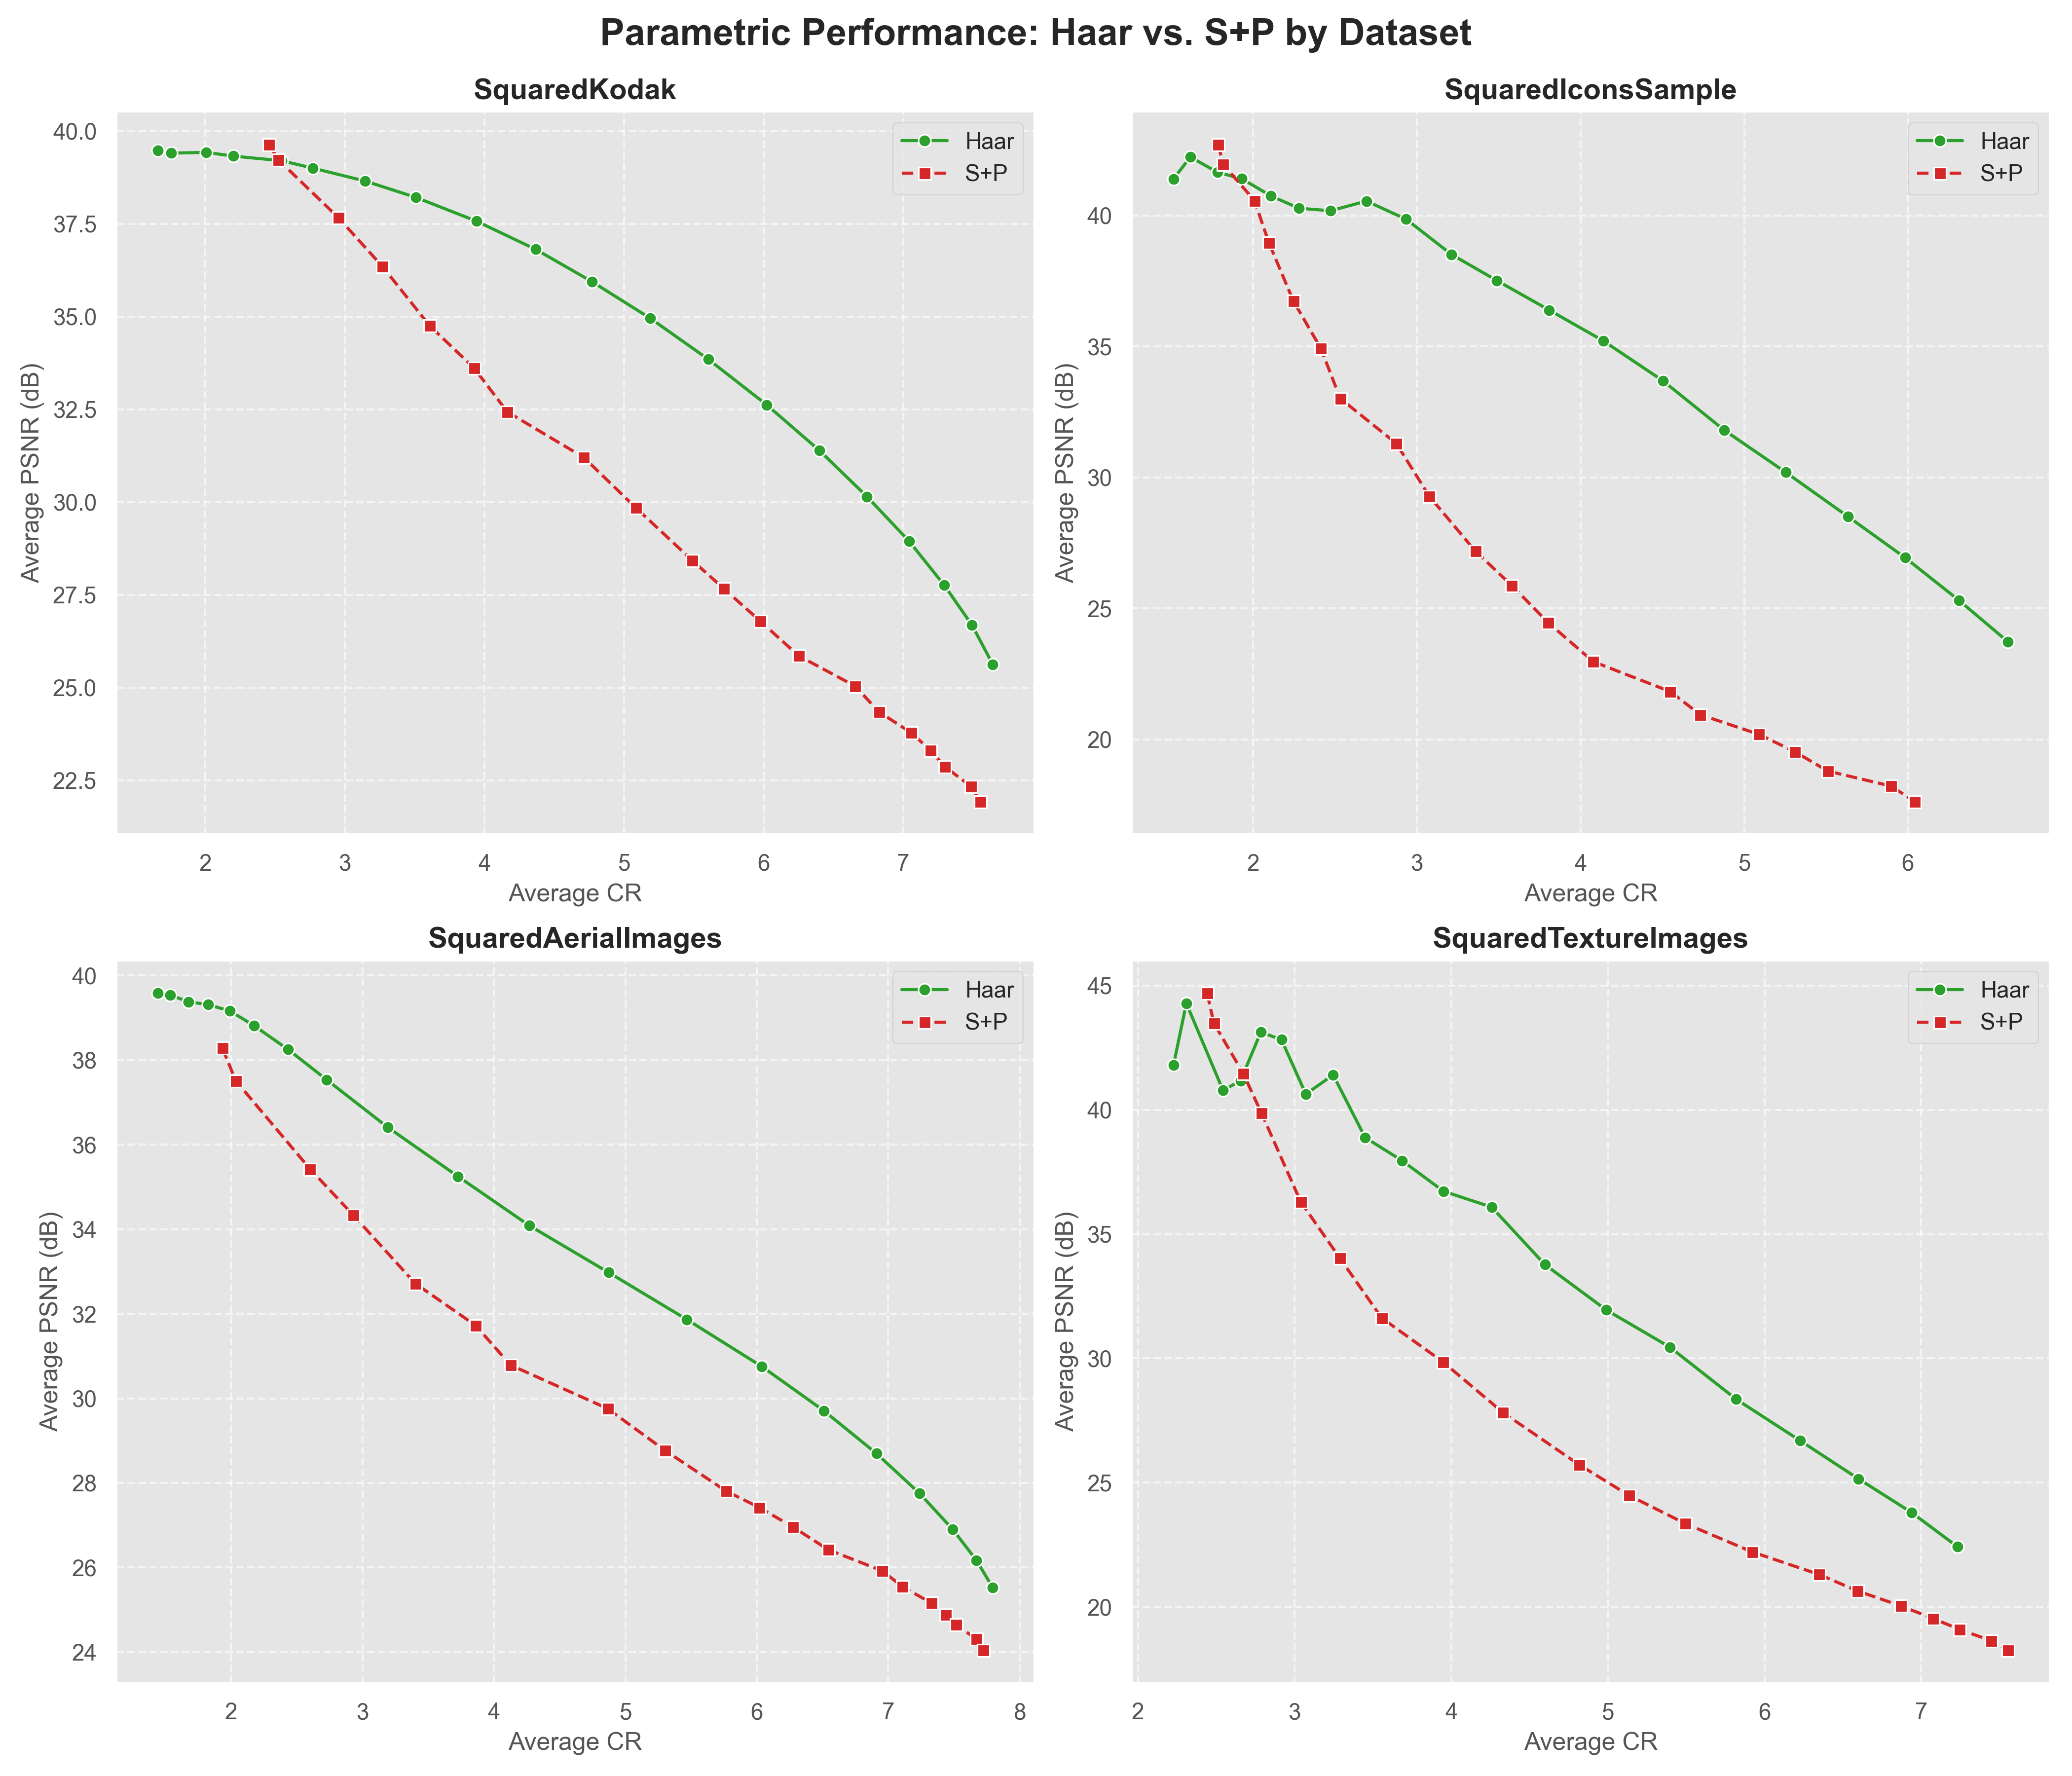
\includegraphics[width=1\linewidth]{results/plots/plot_comparison_Haar_vs_SP_2x2.png}
    \caption{S+P parametric performance: average PSNR vs.\ average compression ratio.}
    \label{fig:haar_vs_sp}
\end{figure}


Fig.~\ref{fig:haar_vs_sp} directly compares Haar and S+P on the same CR--PSNR
axes for each squared dataset. In all four panels, both transforms exhibit the
expected monotone tradeoff between compression ratio and average PSNR, but the
two curves separate as CR increases. For Kodak and AerialImages, the Haar and
S+P curves start close together at low compression ratios (around CR
$\approx 2$ with PSNR near 39–40\,dB), after which the S+P PSNR decreases more
rapidly, yielding several dB lower PSNR than Haar at medium and high CR. A
similar pattern appears for IconsSample and TextureImages: at the lowest CR
values S+P is comparable to Haar (and slightly higher at one operating point
for textures), but beyond roughly CR $\approx 2$ the S+P curve bends downward
more steeply, while the Haar curve remains higher and extends further into the
high-CR regime.

